
\begin{figure}
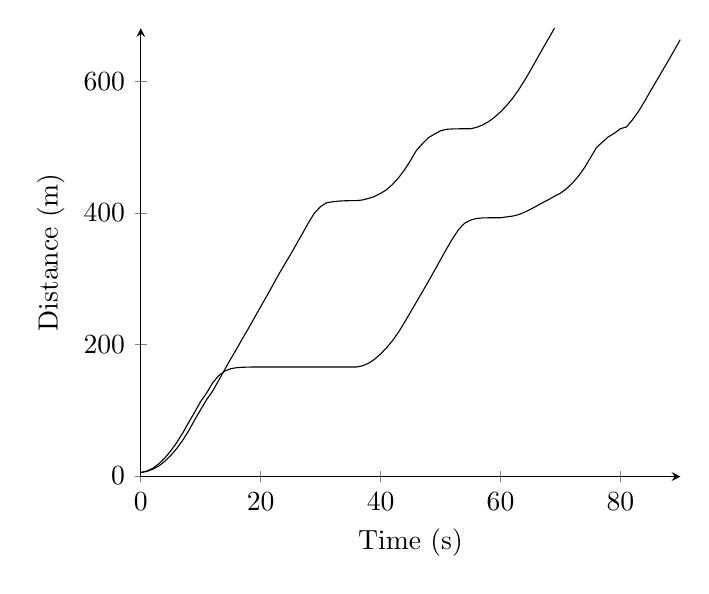
\begin{tikzpicture}
\begin{axis}[
legend style={anchor=west},
axis x line=bottom,
axis y line=left,
ymin=-1,
xlabel=Time (s),
ylabel=Distance (m),
]
\addplot[] coordinates {
(0, 5.1)
(1, 6.83189014051)
(2, 10.0728193274)
(3, 15.0010019455)
(4, 22.1688444693)
(5, 31.025468257)
(6, 41.6438159098)
(7, 54.2803760175)
(8, 68.7630309353)
(9, 85.3336920806)
(10, 100.93621012)
(11, 116.384135557)
(12, 129.208319111)
(13, 145.556731715)
(14, 161.730442812)
(15, 177.986157097)
(16, 193.357529498)
(17, 209.580865522)
(18, 225.122446995)
(19, 241.356740634)
(20, 257.632158281)
(21, 273.552392168)
(22, 289.962983187)
(23, 306.463660298)
(24, 322.008860596)
(25, 337.349714196)
(26, 353.412008642)
(27, 369.43226169)
(28, 385.808926408)
(29, 400.455804401)
(30, 409.899117883)
(31, 415.726311624)
(32, 417.142174741)
(33, 418.176500407)
(34, 418.643261532)
(35, 418.882526456)
(36, 418.932819469)
(37, 419.962570961)
(38, 422.318579458)
(39, 425.315845006)
(40, 429.852490902)
(41, 435.653808339)
(42, 443.708558762)
(43, 453.766912794)
(44, 465.883594594)
(45, 480.151750974)
(46, 495.76737245)
(47, 505.65821073)
(48, 514.882838218)
(49, 520.212615737)
(50, 525.192621044)
(51, 527.435967691)
(52, 528.008829018)
(53, 528.211837632)
(54, 528.253714897)
(55, 528.253714897)
(56, 530.443390002)
(57, 533.975867093)
(58, 539.062235566)
(59, 545.733106434)
(60, 553.946637353)
(61, 563.507416377)
(62, 574.420545771)
(63, 587.297043942)
(64, 601.730368647)
(65, 617.206936625)
(66, 633.448859945)
(67, 649.674063484)
(68, 665.417581111)
(69, 681.282579869)
};
\addplot[] coordinates {
(0, 5.1)
(1, 7.30342432702)
(2, 11.6014519595)
(3, 18.348424014)
(4, 27.138857275)
(5, 37.9783062735)
(6, 50.7236503084)
(7, 65.2145549046)
(8, 81.6747612898)
(9, 97.1218064813)
(10, 113.479606781)
(11, 126.361345892)
(12, 141.734300977)
(13, 152.518181152)
(14, 159.347997992)
(15, 163.094258939)
(16, 164.719958121)
(17, 165.293627152)
(18, 165.577097703)
(19, 165.740681251)
(20, 165.753298313)
(21, 165.753298313)
(22, 165.753298313)
(23, 165.753298313)
(24, 165.753298313)
(25, 165.753298313)
(26, 165.753298313)
(27, 165.753298313)
(28, 165.753298313)
(29, 165.753298313)
(30, 165.753298313)
(31, 165.753298313)
(32, 165.753298313)
(33, 165.753298313)
(34, 165.753298313)
(35, 165.753298313)
(36, 165.753298313)
(37, 167.56057068)
(38, 171.53932787)
(39, 177.562858938)
(40, 185.50778015)
(41, 195.065017632)
(42, 206.006805598)
(43, 218.90324512)
(44, 233.830584072)
(45, 249.310002171)
(46, 265.026069003)
(47, 280.745377392)
(48, 296.406147602)
(49, 312.74384662)
(50, 329.133968477)
(51, 345.504034194)
(52, 361.026724144)
(53, 374.746407133)
(54, 384.502162059)
(55, 389.279465285)
(56, 391.775450371)
(57, 392.580031453)
(58, 392.792479738)
(59, 392.822549576)
(60, 392.822549576)
(61, 394.127315531)
(62, 395.318876876)
(63, 397.564154764)
(64, 401.230303394)
(65, 405.759808388)
(66, 410.588769599)
(67, 415.71529541)
(68, 420.360524082)
(69, 425.543142628)
(70, 430.277832599)
(71, 437.122921729)
(72, 445.816319927)
(73, 456.231806823)
(74, 469.023906046)
(75, 484.172546516)
(76, 499.66101368)
(77, 508.099800966)
(78, 516.162606673)
(79, 521.47138259)
(80, 528.421674224)
(81, 530.981032649)
(82, 541.887026535)
(83, 554.64207687)
(84, 569.50154026)
(85, 585.424941991)
(86, 601.048883585)
(87, 616.53467896)
(88, 632.158372835)
(89, 648.171438419)
(90, 664.12160256)
};

\end{axis}
\end{tikzpicture}
\label{tik:0:79}
\caption{0 percent diving with GSC on route $79$}
\end{figure}
